% Guide to the code of Robot Agentic (software anomaly detection), for reading away from the computer.
% Compile: latexmk -pdf code_guide.tex
\documentclass[10pt]{article}
\usepackage[T1]{fontenc}
\usepackage[utf8]{inputenc}
\usepackage{lmodern}
\usepackage[a5paper,margin=13mm,top=15mm,bottom=16mm]{geometry}
\usepackage{microtype}
\usepackage{amsmath,amssymb}
\usepackage{xcolor}
\usepackage{array}
\usepackage{booktabs}
\usepackage{tabularx}
\usepackage{enumitem}
\usepackage{titlesec}
\usepackage{tcolorbox}
\usepackage{tikz}
\usetikzlibrary{arrows.meta,positioning,fit}
\usepackage{listings}
\usepackage[hidelinks]{hyperref}
\usepackage{fancyhdr}

\definecolor{accent}{HTML}{4F46E5}
\definecolor{soft}{HTML}{EEF2FF}
\definecolor{warn}{HTML}{FEF3C7}
\definecolor{ink2}{HTML}{475569}
\setlength{\parindent}{0pt}
\setlength{\emergencystretch}{3em}
\setlength{\parskip}{5pt}
\setlist{itemsep=1pt,topsep=2pt,leftmargin=*}
\renewcommand{\arraystretch}{1.2}
\titleformat{\section}{\Large\bfseries\color{accent}}{\thesection}{0.6em}{}
\titleformat{\subsection}{\large\bfseries}{\thesubsection}{0.6em}{}
\titlespacing*{\section}{0pt}{10pt}{4pt}
\titlespacing*{\subsection}{0pt}{8pt}{2pt}
\pagestyle{fancy}\fancyhf{}
\lhead{\small\color{ink2} Robot Agentic: the code explained}\rhead{\small\color{ink2}\thepage}
\renewcommand{\headrulewidth}{0.3pt}
\lstset{basicstyle=\ttfamily\footnotesize,breaklines=true,columns=fullflexible,frame=single,rulecolor=\color{black!20},backgroundcolor=\color{black!3},xleftmargin=2pt,xrightmargin=2pt}

\newcommand{\f}[1]{\texttt{#1}}
\newtcolorbox{why}{colback=soft,colframe=accent!60,boxrule=0.4pt,arc=2pt,left=4pt,right=4pt,top=2pt,bottom=2pt,fontupper=\small}
\newtcolorbox{careful}{colback=warn,colframe=orange!70!black,boxrule=0.4pt,arc=2pt,left=4pt,right=4pt,top=2pt,bottom=2pt,fontupper=\small}
\newcommand{\filehead}[2]{\par\smallskip\noindent{\bfseries\ttfamily #1}\hfill{\small\color{ink2}#2 lines}\par\nobreak}

\begin{document}

\begin{titlepage}
\vspace*{18mm}
{\Huge\bfseries\color{accent} Robot Agentic}\par
\vspace{4pt}
{\LARGE The code explained}\par
\vspace{10pt}
{\large Software anomaly detection on URSim: what each part does, how it was built, which libraries and why, how big it is, and what is still missing.}\par
\vfill
Branch \f{refactor/software-detection}, 9 commits on top of \f{main}\par
State of the code on 1 November 2026\par
\vspace{6pt}
{\small\color{ink2} Written to be read on a phone or a tablet: A5 pages, one idea per section. Words in \f{typewriter} are names in the code; the glossary at the end explains the robot words.}
\vspace*{10mm}
\end{titlepage}

\tableofcontents
\newpage

% ---------------------------------------------------------------------------------------------
\section{The project in one page}

\textbf{The goal.} When an industrial robot breaks down, a technician looks at what the robot
reports, makes hypotheses, tests them, and finds the cause. Robot Agentic does the same thing
with an AI agent (Claude). It reads the robot's \textbf{four data sources}:
\begin{enumerate}
\item the \textbf{signals}: joint positions, speeds, currents, torques, temperatures, 500 times per second;
\item the \textbf{logs}: the text lines the robot's programs write;
\item the \textbf{fault codes}: the official error numbers of the controller (e.g.\ \f{C209A0});
\item the \textbf{documentation}: the official manual pages.
\end{enumerate}
It then runs small, slow, operator-approved tests on the robot, and hands in a report:
\emph{the root cause, the evidence, the repair}.

\textbf{Two independent approaches.} You defined two ways of detecting anomalies, that never
mix in one investigation:
\begin{itemize}
\item \textbf{software anomaly detection}: uses only what the robot's software reports (the four sources above). \emph{This is the only one in the code today.}
\item \textbf{physical anomaly detection}: uses our own sensors (microphone, accelerometer, current clamp) on the machine, even a closed one. Planned for later (fan first, then the RoArm-M2-S).
\end{itemize}

\textbf{The test bench.} We do not have a real Universal Robots arm. We use \textbf{URSim}, the
official simulator from Universal Robots: the real controller software, running in a Docker
container on the laptop. To the code, URSim looks exactly like a real UR3e robot: same network
ports, same binary formats, same logs.

\textbf{Two ways to use the agent.}
\begin{itemize}
\item \f{robot-agentic check}: a spot check, on demand (``is the robot OK?''), or a question (``the arm struggles when lifting'').
\item \f{robot-agentic loop}: continuous monitoring. Simple rules (no AI, no cost) watch the logs and fault codes; when something looks wrong, the operator is asked whether to start an investigation.
\end{itemize}
And \f{robot-agentic health} checks that everything is connected.

% ---------------------------------------------------------------------------------------------
\section{The big picture}

The code is cut into four layers. Each layer only knows the one below it.

\begin{center}
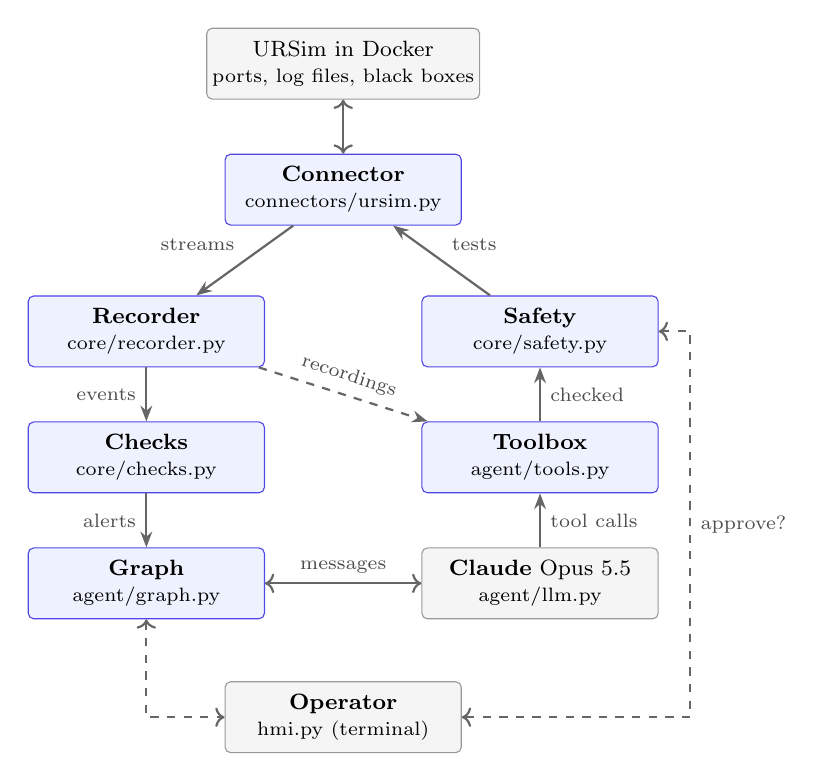
\begin{tikzpicture}[
  box/.style={draw=accent,fill=soft,rounded corners=2pt,align=center,font=\footnotesize,minimum width=30mm,minimum height=9mm,inner sep=2pt},
  ext/.style={draw=black!40,fill=black!4,rounded corners=2pt,align=center,font=\footnotesize,minimum width=30mm,minimum height=9mm,inner sep=2pt},
  arr/.style={-{Stealth[length=2mm]},thick,color=black!60},
  lab/.style={font=\scriptsize,color=black!70}]
\node[ext] (ursim) at (0,0) {URSim in Docker\\\scriptsize ports, log files, black boxes};
\node[box] (conn) at (0,-1.6) {\textbf{Connector}\\\scriptsize connectors/ursim.py};
\node[box] (rec) at (-2.5,-3.4) {\textbf{Recorder}\\\scriptsize core/recorder.py};
\node[box] (safety) at (2.5,-3.4) {\textbf{Safety}\\\scriptsize core/safety.py};
\node[box] (checks) at (-2.5,-5.0) {\textbf{Checks}\\\scriptsize core/checks.py};
\node[box] (tools) at (2.5,-5.0) {\textbf{Toolbox}\\\scriptsize agent/tools.py};
\node[box] (graph) at (-2.5,-6.6) {\textbf{Graph}\\\scriptsize agent/graph.py};
\node[ext] (claude) at (2.5,-6.6) {\textbf{Claude} Opus 5.5\\\scriptsize agent/llm.py};
\node[ext] (op) at (0,-8.3) {\textbf{Operator}\\\scriptsize hmi.py (terminal)};
\draw[arr,<->] (ursim) -- (conn);
\draw[arr] (conn) -- node[lab,above left]{streams} (rec);
\draw[arr] (safety) -- node[lab,above right]{tests} (conn);
\draw[arr] (rec) -- node[lab,left]{events} (checks);
\draw[arr] (checks) -- node[lab,left]{alerts} (graph);
\draw[arr,<->] (graph) -- node[lab,above]{messages} (claude);
\draw[arr] (claude) -- node[lab,right]{tool calls} (tools);
\draw[arr] (tools) -- node[lab,right]{checked} (safety);
\draw[arr,dashed] (rec) -- node[lab,above,sloped]{recordings} (tools);
\draw[arr,dashed,<->] (graph) |- (op);
\draw[arr,dashed,<->] (safety.east) -- ++(0.4,0) |- node[lab,pos=0.25,right]{approve?} (op.east);
\end{tikzpicture}
\end{center}

\begin{enumerate}
\item \textbf{The connector} is the only part that knows URSim. It turns raw bytes and text into
four simple Python types: \f{Sample}, \f{LogLine}, \f{FaultCode} and \f{Recording}.
\item \textbf{The core} (no AI, no robot brand): the \textbf{recorder} keeps the last two minutes of
every stream in memory; the \textbf{checks} raise alerts; the \textbf{safety} layer refuses or
asks before any movement.
\item \textbf{The agent}: the \textbf{graph} drives an investigation, the \textbf{toolbox} runs
what Claude asks for, \textbf{context} turns recordings into plots and tables, \textbf{llm}
talks to Claude.
\item \textbf{Around it}: the command line, the terminal interface, the settings, the
documentation search; and outside the package, the fault-injection tools, the benchmarks
and the tests.
\end{enumerate}

\begin{why}
\textbf{Why this cut?} Plugging in a new machine (the RoArm-M2-S, a car through OBD-II\ldots)
means writing one new connector file. Nothing else changes, because the rest of the code only
knows the four simple types and the \f{Connector} contract.
\end{why}

% ---------------------------------------------------------------------------------------------
\section{How a run goes, step by step}

\subsection{\f{robot-agentic check "the arm struggles"}}
\begin{enumerate}
\item \f{\_\_main\_\_.py} reads the settings (\f{.env}), creates the URSim connector, starts
the recorder (three background threads read signals, logs and fault codes), and builds the
toolbox.
\item The graph starts at the \f{investigate} step. It sends Claude a first message with what
it would ask for anyway: the request, the robot state, the fault codes and the log warnings of
the last two minutes.
\item Claude thinks, then calls tools: e.g.\ \f{search\_docs("C209")}, then
\f{joint\_test(joint=1, delta\_deg=3)}.
\item For a test, the safety layer checks the bounds (±5° max), asks the operator
``\emph{The agent wants to run joint\_test(joint=1, delta\_deg=3). Allow?}'' and the PIN once.
\item The connector sends a tiny URScript program to the robot; the recorder cuts out
everything that happened from 1\,s before to 1.5\,s after the test.
\item Claude receives three things: a text summary (stream cuts, fault codes, log warnings),
a plot of the channels that moved most, and the full values as a table.
\item This repeats (25 turns maximum) until Claude calls \f{submit\_report}. The report is
saved as JSON in \f{data/reports/} and shown in the terminal, with the cost of the calls.
\end{enumerate}

\subsection{\f{robot-agentic loop}}
\begin{enumerate}
\item The graph starts at \f{watch}: it reads every new log line and fault code. No Claude call,
no cost.
\item The \f{EventWatcher} rules decide if an event is an alert (a fault code, a dangerous
phrase like ``protective stop'', or an ERROR line).
\item The operator is asked: ``\emph{Anomaly: fault code C209A0. Start a root-cause analysis?}''
\item If yes: the same investigation as above, then monitoring resumes. Events that arrived
during the investigation are dropped (they were mostly caused by the agent's own tests).
\end{enumerate}

\subsection{\f{robot-agentic health --api}}
One line per check, \(\checkmark\) or \(\times\): Dashboard reachable and robot RUNNING,
Real-Time stream with its rate and channel count, log stream, fault stream, documents found,
and (with \f{--api}) access to the Claude model, through a free API request.

% ---------------------------------------------------------------------------------------------
\section{Languages, libraries and tools, and why}

\subsection{Inside the program}
\begin{center}\small
\begin{tabularx}{\linewidth}{@{}>{\bfseries}l X@{}}
\toprule
Python 3.11+ & The language of robotics and AI tooling; every library below exists for it; it runs on the Raspberry Pi. \\
anthropic (2.3) & Official Claude SDK. Handles retries, authentication (API key or \f{ant auth login}), and the newer features we use: adaptive thinking, effort, prompt caching, server fallback. \\
LangGraph (1.2) & Describes the investigation as a small graph (watch \(\to\) ask \(\to\) investigate \(\to\) report). You chose to keep it: the flow is visible, and adding a step later (e.g.\ ``ask a human expert'') is one node. \\
numpy (2.5) & The ring buffer of signals (one big array), resampling, cut detection. 500 samples/s \(\times\) 63 channels is too much for plain Python objects on a Pi. \\
matplotlib (3.11) & Draws the plot sent to Claude after each test (PNG, in memory). \\
pypdf (6.21) & Reads PDF manuals to index them, if PDFs are added to \f{manuals/}. \\
python-dotenv & Reads the \f{.env} file (API key, robot address, PIN). \\
PyYAML & Reads the scenarios, the catalogue sources (and later the detection thresholds). \\
\bottomrule
\end{tabularx}
\end{center}

\subsection{Python's own library (no install)}
\f{socket} and \f{struct} (talk to the robot's ports and decode its binary packets),
\f{subprocess} (run \f{docker} commands), \f{threading} and \f{queue} (the three reader
threads), \f{dataclasses} (the simple types), \f{zipfile} (open black boxes), \f{gzip}/\f{json}
(save recordings), \f{logging}, \f{argparse} (command line).

\subsection{For development}
\begin{center}\small
\begin{tabularx}{\linewidth}{@{}>{\bfseries}l X@{}}
\toprule
pytest (9.1) & 24 automatic tests, run in seconds, with no robot, no network and no cost. \\
ruff (0.17) & Checks style, imports, \emph{and} the two rules of CONTRIBUTING.md that a tool can check: type annotations and docstrings everywhere. \\
setuptools & Packages the project so that \f{pip install -e .} creates the \f{robot-agentic} command. \\
\bottomrule
\end{tabularx}
\end{center}

\subsection{Outside the program}
\begin{center}\small
\begin{tabularx}{\linewidth}{@{}>{\bfseries}l X@{}}
\toprule
Docker & Runs URSim (image \f{universalrobots/ursim\_e-series}, version 5.26.1). Also the tool to provoke faults: pause, CPU limit, network disconnect. \\
Alpine helper image & 19\,MB image with \f{tc} and \f{iptables}, joined to URSim's network to add delay, loss or block a port. URSim's image has neither tool. \\
udisks & Attaches the 512\,MB disk file URSim runs on, without admin rights, so ``disk full'' never fills the laptop. \\
LaTeX & The fault catalogue and this guide. \\
\bottomrule
\end{tabularx}
\end{center}

\subsection{What was \emph{not} used, on purpose}
\begin{itemize}
\item \textbf{pydantic} (validated models): too slow at 500 samples/s, and each connector already parses strictly. Plain dataclasses instead.
\item \textbf{pandas}: heavy for a Raspberry Pi; numpy is enough.
\item \textbf{A vector database / embeddings} for the documentation: fault codes and part names are exact words, which classic keyword ranking (BM25) handles better, with zero dependency and zero cost.
\item \textbf{LangChain} or an agent framework around Claude: the loop is 60 lines and fully visible; LangGraph is used only for the flow.
\item \textbf{The UR RTDE library}: we read the Real-Time port directly with \f{struct}, which needs no extra package and works the same on a Pi.
\end{itemize}

% ---------------------------------------------------------------------------------------------
\section{The core: \f{src/robot\_agentic/core/}}

These five files know nothing about Universal Robots or Claude.

\filehead{events.py}{123}
The shared vocabulary. Every other file speaks in these types:
\begin{itemize}
\item \f{Sample}: one instant of the signal stream, a time \f{t} and a dictionary
\f{\{"joint\_2\_current\_actual": 0.41, \ldots\}}.
\item \f{LogLine} (time, level, source, text) and \f{FaultCode} (time, code, message, level).
\item \f{Level} (DEBUG to FATAL) and \f{Severity} (warning, critical).
\item \f{Alert}: what wakes the agent up, with its evidence.
\item \f{Param} and \f{ToolSpec}: how a connector describes a test, e.g.\ ``\f{joint}: integer 0--5,
\f{delta\_deg}: number \textminus{}5 to 5, moves the machine''.
\end{itemize}
\begin{why}
The bounds of a test are written \emph{once}, in its \f{Param}. They are shown to Claude (as
\f{minimum}/\f{maximum} in the tool's JSON schema) \emph{and} enforced by the safety layer, so
the two can never disagree.
\end{why}

\filehead{interfaces.py}{69}
The \f{Connector} contract: what every machine must offer. Three streams (\f{signals()},
\f{logs()}, \f{faults()}), \f{docs()}, \f{tools()}, \f{call\_tool()}, \f{stop()},
\f{health()}, and an optional \f{snapshot()} (current state). It is an abstract base class:
Python refuses to create a connector that forgets one method.

\filehead{recorder.py}{305}
The memory of the system.
\begin{itemize}
\item \f{Recorder} starts one thread per stream. If a stream breaks (robot off, network cut), the
thread waits one second and reconnects; the cause is kept in \f{errors}, because a lost stream
is itself a clue.
\item The signals go into a \textbf{ring buffer}: one numpy array of 60\,000 rows (120\,s at
500\,Hz) where the newest row overwrites the oldest. 120\,s on 63 channels is about 60\,MB
instead of more than 200\,MB with one Python object per sample.
\item \f{window(t0, t1)} cuts any time slice out of the buffers into a \f{Recording};
\f{record(action)} runs a test and keeps 1\,s before and 1.5\,s after it. Because the buffer
is always filling, the start of a test is never missed.
\item \f{subscribe()} gives a queue that receives every new log line and fault code: this is
what the loop mode watches.
\item \f{stop()} ends the threads cleanly (added after a bug: leftover threads polluted the
fault captures).
\item \f{Recording} can \f{resample} (average down to fewer points per second, which keeps short
peaks), \f{save} to \f{.json.gz} and \f{load}.
\end{itemize}

\filehead{checks.py}{87}
The rules without AI.
\begin{itemize}
\item \f{EventWatcher.feed(event)}: a fault code always gives an alert; a log line containing
``protective stop'', ``emergency stop'', ``lost communication'', ``connection lost'',
``fault'' (as a whole word, so ``default'' does not match), ``collision'' or ``overcurrent''
gives a critical alert; any ERROR line gives a warning. The same reason is reported at most
once every 30\,s, so a repeating failure does not flood the operator.
\item \f{stream\_gaps(recording)}: the holes longer than 0.1\,s in the signal stream,
including a stream that stops for good before the end of the window.
\end{itemize}
This is where the signal rules (b, e, a, c) will go.

\filehead{safety.py}{76}
Every action Claude asks for passes here first. \f{SafetyPolicy.check}:
\begin{enumerate}
\item every argument must be present, be a number, and be inside its range; otherwise it is
refused (never silently clamped) and Claude is told why;
\item if the action moves the robot: the operator is asked, \emph{every time};
\item if a PIN is configured: it is asked before the first movement of each investigation.
\end{enumerate}
\begin{why}
Even if Claude makes a mistake or is manipulated by a strange log line, the robot cannot leave
limits fixed in advance by humans. Claude only sees ``REFUSED: \ldots'' and has to adapt.
\end{why}

% ---------------------------------------------------------------------------------------------
\section{The URSim connector: \f{connectors/ursim.py}}
\filehead{ursim.py}{672}
The biggest file, on purpose: it is the only place that knows the Universal Robots formats
(your decision: one file). It reads in order, top to bottom.

\subsection{The robot's doors (network ports)}
\begin{center}\small
\begin{tabularx}{\linewidth}{@{}l l X@{}}
\toprule
\textbf{Port} & \textbf{Name} & \textbf{What we do with it} \\
\midrule
30003 & Real-Time & Read the signals: one binary packet every 2\,ms (500\,Hz). \\
30001 & Primary & Read the fault codes (``Robot Message'' packets). \\
30002 & Secondary & Send URScript programs (the robot's language) for the tests. \\
29999 & Dashboard & Text commands: robot mode, safety status, power on, unlock a protective stop. \\
\bottomrule
\end{tabularx}
\end{center}

\subsection{Reading the signals}
\f{\_packets} splits the byte stream into packets (each starts with its own size).
\f{parse\_realtime} reads, at fixed positions in the packet (the table \f{REALTIME\_FIELDS},
from the official ``Remote Control via TCP/IP'' document), 16 groups of values: target and
actual joint positions, speeds, currents, target torques, hand pose and force, motor
temperatures, robot mode, safety mode, accelerometer, speed scaling, voltages. Each becomes a
named channel such as \f{joint\_1\_current\_actual}.

\subsection{Reading the fault codes}
\f{parse\_primary} decodes three message types: error codes, ``key'' messages at level ERROR or
above, and runtime exceptions of a program. A code is written as on the robot's tablet:
\f{C209A0} (code 209, argument 0). Messages replayed by the controller during the first second
of a connection are skipped (they are old).

\subsection{Reading the logs}
There are three log files inside the container: the controller's (\f{URControl.log}), the user
interface's (\f{polyscope.log}) and the teach pendant's event list (\f{log\_history.txt}, what a
technician sees on the tablet). \f{logs()} runs \f{tail -F} on the three through
\f{docker exec}, the way one would read them over SSH on a real controller.

\f{parse\_log\_line} recognises the file from the line's date format, removes colour codes and
NUL characters, extracts the level, keeps multi-line Java messages together, and demotes the
noise of client connections (including ours) to DEBUG so it never raises an alert.

\begin{careful}
A trap found during the study: killing our \f{docker exec} did not stop the \f{tail} inside the
container. The fix: \f{tail} runs in the background of a small shell that waits on our input;
when we stop, the input closes and the shell kills \f{tail}.
\end{careful}

\subsection{The black boxes}
On every error, the robot writes a ``flight report'': a zip with about 30\,s of its own data at
500\,Hz (181 columns, more than the live stream: \emph{target current}, deviation ratios,
payload), and its logs. \f{read\_flight\_report} turns it into a normal \f{Recording}, renaming
columns to the live-stream names so Claude compares like with like, and aligning the time on the
report's ``Reporting Time''. The tool \f{get\_flight\_report(index)} copies one out of the
container; an unreadable one (e.g.\ written on a full disk) gives a clear message instead of a
crash.

\subsection{The tests offered to Claude}
\begin{center}\small
\begin{tabularx}{\linewidth}{@{}>{\ttfamily}l X@{}}
\toprule
joint\_test & One joint turns ±5° max at 10\,\% speed, and comes back. \\
move\_hand & The hand moves ±2\,cm max in a straight line, and comes back. \\
add\_load & Declares up to 1.5\,kg more payload, repeats a shoulder test, restores the original payload (even after an interruption, through \f{recover\_robot}). \\
overall\_test & Each joint in turn, 1--5°: compare the joints with each other. \\
recover\_robot & Close popups, unlock a protective stop, power on, release brakes. \\
get\_flight\_report & Open a black box. Does not move the robot. \\
\bottomrule
\end{tabularx}
\end{center}
Each test is written in URScript (\f{send\_script}), started, and its end is detected by asking
the Dashboard ``running?'' every 0.1\,s (60\,s timeout, then an emergency \f{stopj}).

\begin{why}
\textbf{Why does \f{add\_load} read and restore the payload?} A wrong payload declaration may be
the very fault under investigation. Overwriting it with a fixed value would erase the evidence.
\end{why}

\filehead{fake.py}{136}
A fake six-joint arm in pure Python (100\,Hz), used by the tests: realistic currents (gravity +
speed \(\times\) friction), one \f{joint\_test}, and \f{inject("friction")} or
\f{inject("fault")} to simulate a problem. Fast, free and reproducible.

% ---------------------------------------------------------------------------------------------
\section{The agent: \f{src/robot\_agentic/agent/}}

\filehead{graph.py}{251}
The course of an investigation, as a LangGraph graph with four steps:
\begin{center}\small
\f{watch} \(\xrightarrow{\text{alert}}\) \f{ask\_approval} \(\xrightarrow{\text{yes}}\) \f{investigate} \(\to\) \f{report}
\end{center}
\f{investigate} is the heart: the conversation with Claude. At each turn Claude answers with
thinking, text and tool calls; the tools run; their results are added; and again, until
\f{submit\_report} or 25 turns. If Claude answers without any tool, it is reminded to conclude.
A failing tool returns its error to Claude instead of crashing the investigation.

\begin{why}
\textbf{The conversation is only ever extended, never edited.} This is what makes prompt
caching work (each turn only pays full price for its new part) and keeps Claude's reasoning
from one turn to the next.
\end{why}
\f{run\_check} and \f{run\_loop} are the two modes of section 3.

\filehead{tools.py}{239}
The \f{Toolbox}: the list of tools Claude can call and the code that runs them.
\begin{itemize}
\item Common tools (any machine): \f{get\_status}, \f{get\_recent\_logs}, \f{get\_recent\_faults},
\f{search\_docs}, \f{get\_recording} (a recording as a table, or \f{"latest:N"} for the last
N seconds), \f{plot\_recording}, \f{submit\_report}.
\item Machine tools come from the connector and always go through the safety layer.
\item \f{submit\_report} uses a strict JSON schema: root cause, confidence, evidence, repair,
references, tests done. Claude cannot hand in a report with a field missing.
\item \f{describe\_test}: what Claude gets after each test (summary + plot + full table).
\end{itemize}

\filehead{context.py}{113}
How a recording is shown to Claude without exceeding the budget (\f{RECORDING\_TOKEN\_BUDGET},
40\,000 tokens by default).
\begin{itemize}
\item \f{moving\_channels}: the channels that vary, ranked by how much (range divided by
size, so radians, amperes and degrees can be compared). Constant channels are left out.
\item \f{plot}: up to 8 channels, one per row, as a PNG.
\item \f{csv\_within\_budget}: the table at the finest rate that fits; the rate is halved until
it fits. A 5\,s test at 500\,Hz on 63 channels is 160\,000 numbers, far too many.
\end{itemize}
\begin{why}
\textbf{Why a plot \emph{and} a table?} Research (Zhou \& Yu, ICLR 2025) shows LLMs spot
anomalies in time series better on an image than in a list of numbers. The table keeps the exact
values for checking. You chose to give both.
\end{why}

\filehead{llm.py}{141}
\f{ClaudeClient.create}: one call to Claude Opus 5.5 with
\begin{itemize}
\item \textbf{adaptive thinking} (Claude decides how much to think; a summary is shown in grey);
\item \textbf{effort high} (your choice: a diagnosis needs rigour);
\item \textbf{prompt caching}: a cache point on the system prompt plus automatic caching of the
conversation, so a 20-turn investigation does not pay 20 times for the same history;
\item \textbf{server fallback}: if the model declines, another model answers, and a warning says so.
\end{itemize}
Each call is appended to \f{data/llm\_calls.jsonl} with its tokens, cost and duration.
\f{cost\_usd} computes the price from the public rates (\$4 / \$20 per million input / output
tokens for Opus 5.5).

\filehead{prompts/system.md}{27}
The agent's instructions, in plain English: what it has (four sources, tests, black boxes), the
method (facts \(\to\) ranked hypotheses \(\to\) the smallest test that separates them \(\to\)
conclude), and the rules (no repeating a refused test, check one sensor against another, a
communication failure is a root cause in itself, quote every claim).

% ---------------------------------------------------------------------------------------------
\section{Around the agent}

\filehead{\_\_main\_\_.py}{141}
The \f{robot-agentic} command: \f{build\_runtime} assembles everything (also used by the
benchmarks), \f{health} runs the checklist, \f{main} reads the command line. Ctrl+C stops the
robot's movement before exiting, and the total Claude cost is always printed.

\filehead{config.py}{82}
\f{Settings}: robot address, container name, model, token budget, PIN, log level, folders. Each
field is read from the environment variable of the same name in capitals (\f{ROBOT\_HOST}\ldots),
or from \f{.env}. \f{setup\_logging}: everything goes to \f{data/robot\_agentic.log}, only
warnings to the terminal.

\filehead{hmi.py}{77}
The terminal interface (the only file allowed to \f{print}): alerts in red, questions
\f{[y/N]}, the PIN typed without being shown, tool calls in blue, the report. \f{--yes}
answers yes automatically (simulator and benchmarks only).

\filehead{docs.py}{150}
The documentation search.
\begin{itemize}
\item \f{build} cuts each document (PDF, HTML, Markdown, text) into passages of about 1\,500
characters. A Markdown heading always starts a new passage, and long sections repeat their
heading and source address, so every passage can be quoted with its origin. The result is
cached and rebuilt only when a file changes.
\item \f{DocSearch} ranks passages with \textbf{BM25}, the formula of classic search engines:
rare words that appear often in a short passage score high. A code like \f{C204A3} is also
searched as \f{C204}.
\end{itemize}
Today's documentation: the 225 official UR error code pages (software 5.26), downloaded by
\f{tools/fetch\_ur\_docs.py}, each with its web address.

% ---------------------------------------------------------------------------------------------
\section{Outside the package: tools, benchmarks, tests}

\subsection{Fault injection: \f{tools/fault\_injection/}}
\filehead{inject.py}{233}
\f{URSimFaults}: how to provoke and repair each of the 13 faults: wrong payload, invalid
program, protective stop, controller killed, controller frozen, PolyScope frozen, network cut,
CPU starvation, CPU overload, network delay, packet loss, port 30003 blocked, disk full.
\f{wait\_ready} brings the robot back to RUNNING. Usable alone:
\f{python -m tools.fault\_injection.inject wrong\_payload}.

\filehead{capture.py}{207}
Provokes one fault and saves all the evidence: the raw new log lines (read by byte position
and filtered by time), fault codes, mode changes, stream cuts and rate, new black boxes,
Dashboard state, recovery time. One JSON per run in \f{data/catalogue/}. \f{--repeat 5} for
five runs.

\filehead{catalogue.py + catalogue.yaml + catalogue\_template.tex}{234 + 143 + 79}
Builds the fault catalogue PDF. The rule: \emph{nothing observed is written by hand}.
\f{catalogue.yaml} holds only the commands and the verified official sources;
\f{catalogue.py} computes the observed columns from the captures (with ``5/5''-style run
counts) and fills the LaTeX template.

\filehead{netem/Dockerfile}{4}
The Alpine helper image for network faults.

\filehead{scenarios.yaml}{43}
The benchmark scenarios: a fault, the mode (loop or check), and the expected answer (a
sentence for the judge, keyword groups).

\filehead{tools/fetch\_ur\_docs.py}{83}
Downloads the official error code pages into \f{manuals/ursim/}.

\subsection{Benchmarks: \f{benchmarks/run.py}}
\filehead{run.py}{148}
For each scenario: repair the robot, inject the fault, run the agent, grade the root cause
twice (keywords, and a Claude judge answering in a strict JSON format with low effort), repair
the fault. Prints correct diagnoses, mean time and total cost; saves the results in
\f{benchmarks/results/}.

\subsection{Tests: \f{tests/}}
24 tests, run with \f{.venv/bin/python -m pytest}, using the fake arm and a scripted fake
Claude (no network, no cost):
\begin{itemize}
\item \f{test\_agent.py} (5): a full check produces a report; every movement needs approval; an
out-of-range test is refused without moving; loop mode wakes on a fault and asks; loop mode
stops if the operator declines.
\item \f{test\_core.py} (10): safety bounds and PIN, tool schema, watcher (``default'' is not a
``fault''), ring buffer, recorder stop, save/load, a stream that stops for good, settings.
\item \f{test\_ursim.py} (9): Real-Time and Primary packets, the three log formats, colours,
multi-line messages, pendant lines, documentation search, black box reading, Markdown sections.
\end{itemize}

% ---------------------------------------------------------------------------------------------
\section{How it was developed}

\subsection{The code principles (CONTRIBUTING.md)}
\begin{enumerate}
\item \textbf{Type annotations everywhere}: every parameter and return value says its type.
\item \textbf{Docstrings everywhere}: every module, class and function starts with a sentence
saying what it does (your choice). This is why about a quarter of the lines are explanations.
\item \textbf{Deep modules} (J.\ Ousterhout, \emph{A Philosophy of Software Design}): a simple
interface hiding a rich implementation; no tiny functions called once; each file hides one
decision (e.g.\ only \f{ursim.py} knows the UR byte formats).
\item \textbf{Logging}: every module logs; levels have a meaning; secrets are never logged.
\item \textbf{Comments only for the why}, never to paraphrase the code.
\item \textbf{English everywhere}; \f{ruff} and \f{pytest} pass before every commit.
\end{enumerate}

\subsection{The history of this branch}
\begin{center}\small
\begin{tabularx}{\linewidth}{@{}>{\ttfamily}l X@{}}
\toprule
3f6230e & Refactor: software detection only, English, no baselines, no RoArm or physical code, redundancy removed. \\
149501b & URSim study: evidence capture, pendant log, black boxes, stream-cut fixes. \\
22d0ba1 & Official UR error code pages as documentation. \\
55d2ac9 & Four new faults: PolyScope freeze, network cut, CPU starvation, CPU overload. \\
d375ff4 & Network and disk faults; URSim moved to its own small disk. \\
e27d060 & Capture probe for disk full, \f{--repeat}. \\
934bbc3 & Catalogue generator (observed columns computed only). \\
f48d821 & \f{Recorder.stop()}: fixes the polluted captures. \\
f6c35d2 & The fault catalogue (13 faults \(\times\) 5 runs) and the detection ideas. \\
\bottomrule
\end{tabularx}
\end{center}

\subsection{Bugs found by testing on the real simulator}
Each of these was invisible in the unit tests and only appeared on URSim. They are the reason
the study was worth doing before writing detection rules.
\begin{itemize}
\item \f{tail} kept running inside the container after we stopped (fixed in \f{logs()}).
\item A stream that stopped for good was not counted as a cut (fixed in \f{stream\_gaps}).
\item Recorders were never stopped, and their leftover connections added cuts and warnings to
unrelated faults from round 4 on. Fixed, tested, and all 65 captures redone.
\item Log files contain NULs and get rewritten: reading by line number failed; now by byte
position and time.
\item Killing PolyScope stops the whole container (no supervisor), so that fault became a
freeze instead.
\item \f{docker update --cpus 0} does not remove a CPU limit.
\item The mean sample rate looked normal for a stream that had stopped; the catalogue uses the
effective rate (samples received \(\div\) window length).
\end{itemize}

% ---------------------------------------------------------------------------------------------
\section{How big is it?}

\subsection{Lines, by part}
\begin{center}\small
\begin{tabular}{@{}lrrrrr@{}}
\toprule
\textbf{Part} & \textbf{Total} & \textbf{Code} & \textbf{Docstr.} & \textbf{Comm.} & \textbf{Blank} \\
\midrule
Agent package (\f{src/}) & 2\,668 & 1\,532 & 678 & 28 & 430 \\
Fault tools (\f{tools/}) & 759 & 492 & 137 & 19 & 111 \\
Benchmarks & 149 & 107 & 21 & 1 & 20 \\
Tests & 389 & 256 & 47 & 0 & 86 \\
\midrule
\textbf{All Python} & \textbf{3\,965} & \textbf{2\,387} & \textbf{883} & \textbf{48} & \textbf{647} \\
\bottomrule
\end{tabular}
\end{center}
Plus about 820 lines of Markdown, YAML and LaTeX (README, summary, scenarios, catalogue sources
and template, system prompt).

\textbf{The short answer:} the project is \textbf{about 4\,000 lines of Python}, of which
\textbf{about 2\,400 are real code}. The agent itself is \textbf{2\,668 lines in 19 files, 1\,532
of real code}. The rest is explanations (docstrings, your choice), blank lines, and the tools
that build the fault dataset.

\subsection{The agent package, file by file}
\begin{center}\small
\begin{tabular}{@{}lrr@{}}
\toprule
\textbf{File} & \textbf{Total} & \textbf{Code} \\
\midrule
connectors/ursim.py & 672 & 426 \\
core/recorder.py & 305 & 190 \\
agent/graph.py & 251 & 145 \\
agent/tools.py & 239 & 164 \\
docs.py & 150 & 91 \\
\_\_main\_\_.py & 141 & 84 \\
agent/llm.py & 141 & 75 \\
connectors/fake.py & 136 & 72 \\
core/events.py & 123 & 49 \\
agent/context.py & 113 & 48 \\
core/checks.py & 87 & 36 \\
config.py & 82 & 48 \\
hmi.py & 77 & 41 \\
core/safety.py & 76 & 38 \\
core/interfaces.py & 69 & 24 \\
5 \f{\_\_init\_\_.py} files & 7 & 1 \\
\bottomrule
\end{tabular}
\end{center}

\subsection{Compared with \f{main}}
On \f{main}, the agent package was 2\,917 lines in 33 files. It is now 2\,668 lines in 19 files,
\emph{while gaining} the pendant log, the black boxes, the official documentation and many
fixes. The parts that grew are the fault tools (210 \(\to\) 759 lines: 13 faults instead of 5,
plus capture and catalogue) and the tests (273 \(\to\) 389).

% ---------------------------------------------------------------------------------------------
\section{What is missing}

In order of importance for the project.

\subsection{1. The detection rules on the signals}
\f{core/checks.py} only watches logs and fault codes. Rules b (target vs reality), e (joint
effort ratio), a (hardware limits) and c (recent past) are decided but \textbf{not written}, and
\f{config/detection.yaml} does not exist yet. Consequence, measured in the catalogue: in loop
mode, \textbf{4 of the 13 faults raise no alert at all} (wrong payload, controller frozen,
CPU starvation, CPU overload).

\subsection{2. The expected current in the live stream}
Rules b and e need the current the controller \emph{expects}. Today only the black boxes have it
(\f{current\_target}); the live Real-Time stream reads the target torque but not the target
current. Its position in the packet must be checked on URSim first.

\subsection{3. A ``stream health'' rule (proposed rule g)}
An alert when fewer samples arrive than expected, or none. It would catch 8 of the 13 faults
alone, including 3 that the logs miss. Waiting for your decision.

\subsection{4. Benchmarks: never run, and incomplete}
\begin{itemize}
\item \textbf{The agent has not yet done a full investigation with the real Claude on this
branch}: \f{data/reports/} and \f{benchmarks/results/} are empty. Everything in the agent is
tested with a fake Claude only.
\item \f{scenarios.yaml} covers only 5 of the 13 faults.
\item So the statistics (\% detected, \% correct cause, detection time, cost) do not exist yet.
\end{itemize}

\subsection{5. Smaller gaps in the code}
\begin{itemize}
\item The summary Claude gets after a test gives the \emph{mean} rate between the first and last
sample, which can look normal when the stream stopped (the catalogue already uses the
effective rate; the agent should too). The cuts are reported, so it is not hidden, only
misleading.
\item \f{Recorder.subscribe()} has no ``unsubscribe'': each loop scenario of a benchmark adds a
queue that keeps filling. Harmless for one run, a slow memory leak over many.
\item The documentation is only the error code pages: no User or Service Manual yet, so Claude
cannot quote a repair procedure or a hardware limit (which rule a needs).
\item No tests for the fault tools, the benchmark runner, the cost computation or the
plot/table budget; no automatic end-to-end test against URSim; no continuous integration.
\item An old \f{data/baselines/} folder from before the refactor is still on disk (not in git).
\end{itemize}

\subsection{6. Planned for later (summary.md, section 6)}
\begin{itemize}
\item The RoArm-M2-S connector, with log lines and error codes we generate ourselves.
\item Physical anomaly detection: ESP32 \(\to\) USB \(\to\) Raspberry Pi, FFT and rules on the Pi,
Claude explains.
\item Running everything on the Raspberry Pi.
\item An interface other than the terminal (web, notifications), and reports in a readable
format (today: JSON + terminal).
\end{itemize}

% ---------------------------------------------------------------------------------------------
\section{Glossary}
\small
\begin{description}[style=nextline,leftmargin=0pt,itemsep=3pt]
\item[URSim] The official Universal Robots simulator: the real controller software, without the arm.
\item[URControl] The controller program: computes movements, serves ports 30001--30004.
\item[PolyScope] The robot's user interface (on the tablet). Serves the Dashboard (29999) and writes the black boxes.
\item[Teach pendant] The tablet used to program and drive the robot. Its event list is \f{log\_history.txt}.
\item[URScript] The robot's programming language (\f{movej}, \f{set\_target\_payload}\ldots).
\item[Protective stop] The robot stops because a safety limit was crossed; code \f{C209} when triggered by a program.
\item[Robot mode / safety status] e.g.\ RUNNING, POWER\_OFF / NORMAL, PROTECTIVE\_STOP.
\item[Black box (flight report)] Zip written by the robot on each error: ~30\,s of its own data and logs.
\item[Payload] The mass declared for the tool. A wrong value makes the expected torques wrong.
\item[Following error] The gap between the position the controller asked for and the real one.
\item[Ring buffer] A fixed-size memory where new data overwrites the oldest.
\item[BM25] The ranking formula of classic search engines.
\item[Token] The unit Claude reads and is billed by, about 3--4 characters of text.
\item[Prompt caching] Claude's API keeps the start of a conversation in memory, so resending it costs much less (20 times less for Opus 5.5).
\item[Adaptive thinking / effort] Claude decides how long to think; ``effort'' sets how thorough it is.
\item[LangGraph] A library to describe a program's flow as a graph of steps.
\item[netem / iptables] Linux tools to delay or lose network packets / block a port.
\item[Docker container] An isolated mini-system running one program (here URSim) on the laptop.
\end{description}

\end{document}
